41. Перед вами МНОГОУГОЛЬНИК. У него может быть сколько угодно ВЕРШИН. ({\it На предложенном рисунке их всего 6, для примера.}) Представьте себе двадцатиугольник (у него 20 вершин). Одну из его вершин соединим отрезками со всеми остальными. На сколько треугольников мы разделим двадцатиугольник?
\begin{center}
\begin{figure}[ht!]
\center{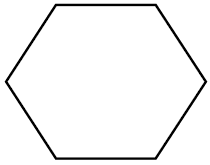
\includegraphics[scale=0.35]{6.png}}
\end{figure}
\end{center}
